\chapter{Conclusion}\label{chapter:conclusion}

This thesis demonstrates several ways to capture distributions of student solutions and make this information useful to teachers and students in large programming classes. Capturing commonalities can save teachers time and exhaustion by summarizing many solutions with a single representative. It can also direct teachers to where the majority of the class is within the space of solutions or errors, so they can respond to student needs based on data, not hunches. Capturing variation allows teachers to see how students deviate from the common choices in ways that are superior and deserving celebration or inferior and requiring corrective feedback. These deviations can be used to inspire or directly seed exercises based on modern theories of how students learn generalizeable knowledge from concrete examples. It also saves teachers the time and effort of generating pedagogically valuable examples themselves. Systems in this thesis also demonstrate how the inherent variation in student solutions can be automatically presented back to students, as an active reflection exercise that can benefit both current and future students. 

The technical challenges tackled in order to capture and display distributions of solutions include designing solution representations, measures of similarity between solutions, mechanisms for grouping or filtering them, and human-interpretable displays. Challenges in workflow design centered around simple, minimally-intrusive ways to perform targeted learnersourcing in an on-going programming class.

\section{Summary of Contributions}

The original OverCode system included a novel visualization that shows similarity and variation among thousands of Python solutions, backed by an algorithm that uses the behavior of variables to help cluster Python solutions and generate human-interpretable normalized code for each cluster of solutions. The Foobaz system demonstrated how, even when an aspect of variation is hidden in one view of a distribution of solutions, it can be exposed, in context, in a separate view. Additional follow-on work expanded OverCode's normalization process to incorrect solutions and explored additional human-interpretable mechanisms for identifying population-level design alternatives.

Foobaz contributed a workflow for generating personalized active learning exercises, emulating how a teacher might socratically discuss good and bad choices with a student while they review the student's solution together. The Foobaz system demonstrates one concrete way in which a conversation about design decisions, i.e., variable naming, that might only happen in one-on-one interactions with an instructor, can be scaled up to an arbitrarily large class, personalized to each student, be based on the distribution of naming choices found in solutions composed by the teacher's current class or previous classes, and deployed to future classes who assign the same programming exercise.

Finally, the self-reflection and comparison workflows demonstrate the potential of targeted learnersourcing. The self-reflection workflow allows students to generate hints for each other by reflecting on an obstacle they themselves have recently overcome while debugging their own solution. The comparison workflow prompts students to generate design hints for each other by comparing their own solutions to alternative designs submitted by other students. Studies of the Dear Beta and Dear Gamma systems show that personalized hints collected through these workflows can be viably learnersourced, and that these hints serve as helpful guides to fellow students encountering the same obstacle or attempting to reach the same goal.

\section{Future Work}
``One never notices what has been done; one can only see what remains to be done...'' - Marie Curie (1984)

There are many directions in which this work can be grown. Some of the research that has been published in parallel with this work can be directly incorporated into future systems. At the same time, many of the existing features can be improved without incorporating any new techniques, based on already collected feedback during user studies, deployments, and other design critiques.

\subsection{OverCode}

OverCode was designed for thousands of correct solutions to introductory Python programming problems. Many residential and online exercises now afford automatic, immediate feedback about the correctness of a solution. Under these conditions, nearly all the final solutions are correct, but it is clear from reading through them that some students have better command of programming than others, just based on compositional quality. As a result, OverCode was designed to reveal to the teacher what their students' solutions actually look like, modulo white space and comments. These solutions are rendered for the teacher using most common variable names and statement orders.\todo{check the statement order} 

However, as programming exercises escalate from the simple to the complex, OverCode's utility breaks down. It can still create normalized cluster-representing solutions and display them in a way that helps teachers spot contrasts, but the clusters themselves become smaller and smaller. As programming exercises require more complex solutions, there is also an increasing need to go beyond representing what students actually wrote and toward human-interpretable representations of larger clusters. There are two promising complementary avenues for implementing this next step.

The first avenue is more bottom-up clustering. Just as the variation in variable names was hidden by recognizing that variables across programs were semantically equivalent and could be replaced with their most popular student-given name, it may be possible to do the same with respect to semantically-equivalent subexpressions. There two promising ways to determine the semantic equivalence of subexpressions or lines of code in large corpuses of student solutions: (1) semantic equivalence based on the rules of the programming language (2) probablistic semantic equivalence based on the dynamic behavior during execution on test cases, as defined in Nguyen et al.~\cite{codewebs}. OverCode could feature an additional button which collapses these detected equivalences, showing the most popular choice in the solution representing the new, larger clusters. An interface, perhaps like the teacher interface in Foobaz, can allow teachers to view and compose feedback that dimension of variation, if they wish. 

The second promising avenue for creating larger clusters is continuing to model the corpus of solutions to the same programming exercise as samples from an underlying distribution of solutions shaped by the teacher's explanations, student's prior knowledge, common novice misconceptions, and the constraints of the language itself. Depending on the model chosen, larger clusters could be groups of whole solutions or groups of sub-components the co-occur within many solutions. Iterating on solution representation, model choice, interface, and interaction will hopefully allow teachers to understand their students' design choices, give style feedback, and assign grades with confidence. 

Even simple additions to the OverCode interface could approximate what more sophisticated statistical methods would do. For example, LDA may pull out distributions of commonly co-occuring variable behaviors (as described in the chapter on OverCode extensions), but the current OverCode interface could be modified to suggest and filter by common sets of strictly co-occurring variable behaviors. This approximation is less robust in the face of noise, but it is at least easier for the user to interpret using the language of filtering. %mechanisms. rather than relying on LDA , applied to identify common types of solutions, the OverCode interface could suggest and support filtering for solutions that have a common set of strictly co-occuring variable behaviors. 

When visualizing the resulting clusters, it is important to keep in mind the ease with which users can interpret the results. Simple modifications to the OverCode interface can go a long way, such as highlighting the sub-expressions or normalized variable names within lines of code, rather than the entire lines, that separate one cluster from another. Another modification would increase the interpretability of the normalized variables. Since the variable behavior is used to normalize variable names, the values of variables and sub-expressions during execution on a test case could be displayed just beneath or alongside the code, as demonstrated in an experimental Python notebook~\cite{kevinkwokdemo}, in addition to the way it is currently shown, as a legend mapping each variable name to its behavior beneath a tab that many user study subjects did not consult. 


%\todo{Interface upgrades: talk about beneath-line value annotation like that cool notebook and showing differences at the level of subexpressions, and filtering by sets of common variables in solutions which is like cheap version of lda on variables}

When the program tracing, renaming, or reformatting scripts generate an error while processing a solution, the solution is removed from the pipeline. This percentage of correct edX solutions that did not make it through the pipeline was less than five percent of solutions were excluded from each problem, but that can be reduced further by adding support for handling more special cases and language constructs to these library functions. As solutions get more complex, it will also be necessary to expand the OverCode pipeline to more gracefully handle user-created objects and helper functions. Complementary efforts, like ~\cite{choudhury2016autostyle}, also cannot yet handle more than a single function. This remains a difficult but important hurdle to expanding beyond introductory Python programming courses. As part of this expansion, it may be helpful to adopt the \texttt{observe} construct introduced by Gulwani et al.~\cite{gulwani_fse14} and support teacher annotation of solutions with the observe construct within the OverCode user interface. By soliciting human annotation of important variable values, two variables would not need to behave identically in order to be considered by OverCode as semantically the same.% reduces the need for variables

OverCode could also be integrated with the autograder that tests student solutions for input-output correctness. The execution could be performed once in such a way that it serves both systems, since both OverCode and many autograders require actually executing the code on specified test cases. If integrated into the autograder, teachers could give feedback by writing line- or stack-specific feedback to be sent to students alongside the input-output test results. The OverCode interface may also provide benefit to students, in addition to teaching staff, after students have solved the problem on their own. Cody is a standing example of the value of this kind of design/style feedback. However, the current interface may need to be adjusted for use by non-expert students, instead of teachers. %This would require pipeline and user interface modifications, in order to account for the fact that not all solutions would be returning the same values for each test case.

Simple interface enhancements would give teachers, and potentially students, more freedom to explore. For example, many user study subjects requested the ability to promote any cluster to be the reference cluster. A student might want to see their solution as the reference, at least as a starting point. Similar to GroverCode's sorting mechanism, the OverCode interface could support sorting clusters by their similarity to the reference as well as by cluster size. 

\todo{add text about boolean variables not being renamable, require more information, perhaps even more than GroverCode collections}

\subsection{GroverCode}

GroverCode's normalization of incorrect solutions is based on heuristics about co-occurrences of syntax and variable behavior in both correct and incorrect solutions. This was an attempt to see how far the OverCode features could go toward normalizing incorrect solutions in addition to correct solutions, without using any additional technology. However, there is pre-existing technology, i.e., AutoGrader~\cite{autograder}, that could be added to the pipeline. 

The AutoGrader understands a language for expressing corrections in introductory Python programs. The authors created a list of such possible corrections, and if applying a small subset of those corrections changes a solution's input-output behavior to match a reference solution, the Autograder can automatically correct the solution. It does not take into account which sets of corrections are more common, unlike the design philosophy the defines OverCode.\todo{check this} However, the corrections that are applied are guaranteed to convert the incorrect solutions into correct ones. The correct solutions can move through the OverCode pipeline to be normalized and clustered without heuristics. 

If the AutoGrader is added to the pipeline, it will likely move some but not all solutions from the incorrect to the correct category. The corrections that have been automatically applied could be displayed alongside the corrected code in the GroverCode interface, for transparency. The GroverCode process for analyzing and displaying solutions that are still incorrect after being analyzed by the AutoGrader would be unchanged. If the language for expressing corrections is simple and expressive enough that it can be used by graders to write new rules while they are grading, the combined AutoGrader-OverCode pipeline could be rerun to correct any other yet ungraded solutions that are not already automatically corrected. 

There are also a variety of interface updates that have also been requested by the teachers who used GroverCode during live deployments, such as the ability to add new tests to the test suite. These requests have been catalogued and added the the project as feature requests. 

\subsection{Foobaz}

%This is a step on a clear path toward user interfaces that allow teachers to give meaningful feedback to students at scale about a variety of at least partially subjective but important aspects of code. We believe that 
The approach taken in designing Foobaz may be generalizable to other aspects of programming style. Just as OverCode establishes the equivalency of variables based on their behavior during test cases, one could establish the behavior equivalency of larger or more abstract entities, such as student-written lines of code, sets of lines of code, or entire functions. We consider this a class of problems that Foobaz, and similar systems built after it, can tackle. Future iterations of Foobaz-inspired interfaces could also include additional constraints and affordances to encourage teachers to leave more explanations for their assessments, accompanied by better support for reusing common comments. Teachers could also be given the option to augment or overwrite existing labels, e.g., ``too short,'' to match their own preferences. %Finally, based on usage logs and Likert scale ratings on the helpfulness of various features, we will simplify the interface by removing unappreciated features and improve average response times by eliminating redundant computation.

\subsection{Targeted Learnersourcing}

The primarily difficulty of iterating on the two workflows, Dear Beta and Dear Gamma, is that they are most successful when they are directly integrated into teacher's own systems and endorsed or promoted by staff. In future classes with supportive teachers, a module can be added to the Dear Beta workflow that identifyies when a student is in a good place to supply a hint and prompts them to do so. This would be an improvement over the current stand-alone website that students are explicitly directed to when they need help, but not when they can give help. Future work on Dear Gamma should include improving the metric for optimality and the rendering of solutions such that all the differences between more and less optimal solutions are visible to reflecting, hint-writing students. One potential future incarnation of the Dear Beta and Dear Gamma workflow is a crowd-sourced intelligent tutor that helps students get to a correct solution and then optimize that solution, completely driven by student-written hints. %To make this happen, the infrastructure to connect these systems to each other and to an existing course needs to be built. 



% on common errors and on strategies to convert less optimal student-written correct solutions into more optimal ones. %ranked by an  We will also explore what Dear Gamma in the context of the software engineering course could look like, e.g., prompting students to write hints about the style and correctness of code written by other students. We plan to continue deploying iterations of these workflows in classes for students' immediate benefit, and to demonstrate that it can enrich the learning experience across multiple engineering domains.

%\todo{use a platform like http://lalitjain.com/files/next.pdf}



%\subsection{Mathematical Expressions}

%they may be able to add new correction rules to the AutoGrader's list as they grade. 

%It is also possible that the gap between automatically corrected solutions and those solutions that could not be automatically corrected could be exposed in the inter

% and has demonstrated  correction rates of ;  have used that language to create an error model for  that can correct incorrect solutions automatically if a small number of items in the error model can; utoGrader searches the space of all possible applications of those 


%two ways come from the field of Bayesian inference, and specifically, latent variable models that find (1) clusters of solutions or (2) topics that cut across solutions. The benefit of the existing OverCode clustering pipeline is that, when looking at the cluster representative solution, the teacher knows exactly which ways the solutions beneath it vary and in which ways they do not. 

%Traditional The challenge of displaying clusters 

%interpretable clustering methods. 

%Latent variable models 



%\todo{skim and add later: "As new solutions are submitted by students, the number of observed distinct student design decisions may grow without bound, and each solution may be a mixture of multiple design decisions. Therefore, a Hierarchical Dirichlet Process \cite{hdp} for learning these underlying design decisions may be a good model choice for this data. However, since some design decisions may be correlated with each other, it may be even more accurate to replace the (conveniently conjugate) Dirichlet prior with a (non-conjugate) logistic normal prior that can model correlated topics in addition to uncorrelated topics. This would be a non-parametric version of the Correlated Topic Model \cite{ctm}. If, as is likely, the chosen features can belong to multiple design decisions, it may be useful to add in elements of the Indian Buffett Process \cite{ibp}. Since (1) we do not know how many clusters will exist in the data ahead of time and (2) new solutions may introduce new clusters (there is no finite limit on the number of clusters as more solutions are received), models built on Dirichlet Processes are a good fit. Since solutions may contain multiple design decisions, it is preferable to be able to assign each of those design decisions separately, rather than assigning the entire solution to a cluster. HDPs are a good fit. If different design decisions share common features, IBPs may be an even better fit.Since the output of LDA and its infinite cousin, the HDP, can be difficult to interpret, BCM or MGM's optimizations for interpretability may make them more appropriate choices.Since teachers develop their own internal rubric for which differences matter and which do not, models which can incorporate and adjust based on feedback from the user, like iBCM, may be good model choices.Each of these models have favorable properties, and some properties can be super-imposed, while others are mutually exclusive. There is also previously ignored factors like the difficulty of implementing an inference algorithm for the model and the scalability and time requirements of running the chosen inference algorithm on the chosen representation of the solutions."}

\begin{comment}

A generative model specifically for this kind of dataset may be worth designing and building around. Encoding solutions in a variable-by-solution matrix only allows the mixture model to separate solutions based on variable behavior. Variable behavior carries a lot of information about how a student approached computing the solution, but this representation ignores the important differences between solutions using, e.g., idiomatic Python or tangled syntax. A pedagogical tool that supports teachers at both levels would be ideal. Adding an additional layer of hierarchy to the LDA plate model might allow for modeling distribution of variables in solutions, as well as the syntax responsible for that behavior.

Consider the plate model of LDA. If one adds one more level of hierarchy, then one level can capture the distribution over combinations of variables in a solution and the next level can capture the distribution over the possible syntax to create the execution behavior that defined those variables. What is observed is a set of lines of syntax that manipulate the variables. Future work includes exploring whether inference based on this generative model is tractable.

\begin{figure}[ht]
%\vskip 0.2in
%\begin{center}
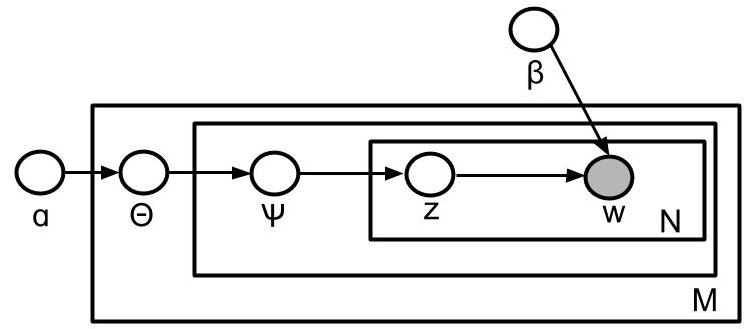
\includegraphics[width=0.75\columnwidth]{figures/LDA_inspired_new_plate_model}
\caption{Alternative plate model for modeling Python solutions}
\label{LDA_inspired_new_plate_model}
%\end{center}
%\vskip -0.2in
\end{figure}


Our user study participants produced a variety of suggestions for additional features. In addition to those but unmentioned by users, variable renaming obscures pedagogically relevant information. The user-tested UI does not include access to raw solutions represented by a stack's cleaned code, or to the original variable names represented by a common variable name. This can be accomplished by adding tooltips and dropdown menus. This may also be part of better communicating to users that they are looking at cleaned, not raw, code.

\end{comment}


%"finger exercises" to exam questions, the complexity of solutions increases. 